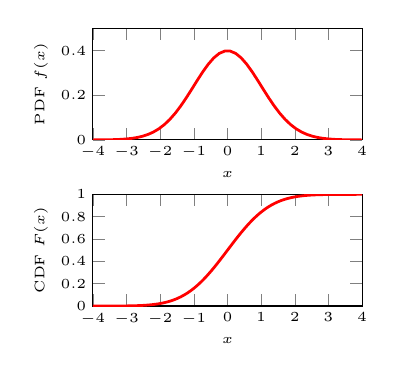
\begin{tikzpicture}
    \tiny
    \begin{axis}[
            width = 5cm,
            height = 3cm,
            % width = \linewidth,
            % unit vector ratio={1 1},
            name = axis1,
            xmin = -4,
            ymin  = 0,
            xmax = 4,
            ymax = 0.5,
            xtick distance=1,
            % ytick={0,3,8},
            % yticklabels={0,$\lambda_1$,$\lambda_2$},
            % xtick = {0},
            % xticklabel=\empty,
            xlabel={$x$},
            ylabel={PDF $f(x)$},
            legend style={at={(1,1)},anchor=north east},
            legend style={font=\tiny},
            grid style=dashed,
            domain=-4:4,
            samples=50,
        ]
        \addplot [
            color=red,
            line width = 1pt,
        ]
        {1/(sqrt(2*pi))*exp(-x^2/2)};
    \end{axis}
    \begin{axis}[
            width = 5cm,
            height = 3cm,
            % width = \linewidth,
            % unit vector ratio={1 1},
            name = axis2,
            xmin = -4,
            ymin  = 0,
            xmax = 4,
            ymax = 1,
            xtick distance=1,
            % ytick={0,3,8},
            % yticklabels={0,$\lambda_1$,$\lambda_2$},
            % xtick = {0},
            % xticklabel=\empty,
            at=(axis1.below south west), anchor=above north west,
            xlabel={$x$},
            ylabel={CDF $F(x)$},
            legend style={at={(1,0)},anchor=south east},
            legend style={font=\tiny},
            grid style=dashed,
        ]
        \addplot [
            color=red,
            line width = 1pt]
        coordinates {
                (-4, 0.00003)
                (-3.9, 0.00005)
                (-3.8, 0.00007)
                (-3.7, 0.00011)
                (-3.6, 0.00016)
                (-3.5, 0.00023)
                (-3.4, 0.00034)
                (-3.3, 0.00048)
                (-3.2, 0.00069)
                (-3.1, 0.00097)
                (-3.0, 0.00135)
                (-2.9, 0.00187)
                (-2.8, 0.00256)
                (-2.7, 0.00347)
                (-2.6, 0.00466)
                (-2.5, 0.00621)
                (-2.4, 0.0082)
                (-2.3, 0.01072)
                (-2.2, 0.0139)
                (-2.1, 0.01786)
                (-2.0, 0.02275)
                (-1.9, 0.02872)
                (-1.8, 0.03593)
                (-1.7, 0.04457)
                (-1.6, 0.0548)
                (-1.5, 0.06681)
                (-1.4, 0.08076)
                (-1.3, 0.0968)
                (-1.2, 0.11507)
                (-1.1, 0.13567)
                (-1.0, 0.15866)
                (-0.9, 0.18406)
                (-0.8, 0.21186)
                (-0.7, 0.24196)
                (-0.6, 0.27425)
                (-0.5, 0.30854)
                (-0.4, 0.34458)
                (-0.3, 0.38209)
                (-0.2, 0.42074)
                (-0.1, 0.46017)
                (0.0, 0.5)
                (0.1, 0.53983)
                (0.2, 0.57926)
                (0.3, 0.61791)
                (0.4, 0.65542)
                (0.5, 0.69146)
                (0.6, 0.72575)
                (0.7, 0.75804)
                (0.8, 0.78814)
                (0.9, 0.81594)
                (1.0, 0.84134)
                (1.1, 0.86433)
                (1.2, 0.88493)
                (1.3, 0.9032)
                (1.4, 0.91924)
                (1.5, 0.93319)
                (1.6, 0.9452)
                (1.7, 0.95543)
                (1.8, 0.96407)
                (1.9, 0.97128)
                (2.0, 0.97725)
                (2.1, 0.98214)
                (2.2, 0.9861)
                (2.3, 0.98928)
                (2.4, 0.9918)
                (2.5, 0.99379)
                (2.6, 0.99534)
                (2.7, 0.99653)
                (2.8, 0.99744)
                (2.9, 0.99813)
                (3.0, 0.99865)
                (3.1, 0.99903)
                (3.2, 0.99931)
                (3.3, 0.99952)
                (3.4, 0.99966)
                (3.5, 0.99977)
                (3.6, 0.99984)
                (3.7, 0.99989)
                (3.8, 0.99993)
                (3.9, 0.99995)
                (4.0, 0.99997)
            };
    \end{axis}
\end{tikzpicture}